\chapter{Sviluppo del progetto di stage}
\label{chap:sviluppo}

\section{Web design}
\noindent L’estensione è stata progettata con un approccio \glslink{desktop-firstg}{\textit{desktop-first\glox}}, in considerazione del target principale costituito da sviluppatori web che operano prevalentemente su schermi di grandi dimensioni. \\Tale scelta consente di privilegiare la chiarezza e l’ampiezza degli spazi di lavoro, garantendo una disposizione ottimale dei pannelli e delle funzionalità principali.\\
Particolare attenzione è stata posta all’accessibilità cromatica, mediante uno studio accurato dei contrasti tra testo, sfondo ed elementi interattivi, al fine di assicurare leggibilità anche in condizioni visive differenti. \\È stata inoltre implementata la possibilità di personalizzare l’esperienza visiva tramite un pulsante dedicato alla selezione della modalità giorno/notte, che permette all’utente di adattare l’interfaccia alle proprie preferenze e alle condizioni ambientali di utilizzo.\\
Nonostante l’approccio iniziale privilegi i dispositivi desktop, il layout rimane responsivo grazie a soluzioni flessibili che mantengono l’usabilità anche su schermi di dimensioni ridotte. Questa scelta assicura un’esperienza coerente ed accessibile in diversi contesti d’uso.

\section{PoC}
\noindent L’obiettivo iniziale era la realizzazione di un \glslink{pocg}{Proof of Concept\glox} (\glslink{poc}{\acrshort{poc}\glox}) che permettesse di verificare la fattibilità tecnica dell’estensione proposta. In questa fase preliminare, l’attenzione era rivolta principalmente a due aspetti fondamentali: il recupero del codice sorgente della pagina web e l’integrazione con un’\acrshort{api} di \glslink{iag}{intelligenza artificiale}, necessaria per avviare i primi test di analisi e generazione di suggerimenti.\\
Il \acrshort{poc} non teneva conto di aspetti come la scalabilità, l’ottimizzazione delle performance o la gestione di casi d’uso complessi, ma si limitava a dimostrare che le funzionalità di base potessero essere effettivamente implementate. 
\\La struttura iniziale era volutamente semplice in quanto conteneva solamente funzioni basilari nei file:
\begin{itemize}
  \item \texttt{script.js}: responsabile dell’avvio dell’estensione;
  \item \texttt{analysis.js}: deputato all’estrazione del codice sorgente della pagina web e alla sua messa a disposizione per ulteriori elaborazioni;
  \item \texttt{service\_worker.js}: gestisce le richieste verso il modello di \glslink{iag}{intelligenza artificiale}, inviando il codice recuperato e ricevendo in risposta i suggerimenti generati.
\end{itemize}

\noindent Questa versione sperimentale costituiva una base minima ma solida su cui successivamente è stato possibile costruire le funzionalità avanzate, affinare l’interfaccia e integrare logiche più complesse per la gestione dei risultati.\\


\section{Prodotto finale}
\noindent In questo paragrafo viene illustrato il risultato concreto del progetto: l’estensione web \textit{SviluppAbile} (logo in figura \ref{fig:logo_sviluppabile}), uno strumento progettato per supportare gli sviluppatori nell’individuazione e nella correzione degli errori di accessibilità nelle pagine web. Di seguito, viene descritta l’estensione realizzata e vengono analizzate le funzionalità implementate, mettendo in evidenza l’integrazione con il \glslink{chatbotg}{chatbot} e le modalità di interazione con l’utente.

\begin{figure}[H]
    \centering
    
\includegraphics[width=0.15\linewidth, alt={Logo dell'estensione \textit{SviluppAbile}}]{img/sviluppabile.png}
    \caption{Logo dell'estensione \textit{SviluppAbile}}\label{fig:logo_sviluppabile}
\end{figure}

\subsection{Guida all'utilizzo}
\noindent La presente sezione illustra le funzionalità dell’estensione attraverso una dimostrazione pratica guidata, supportata da screenshot dell’interfaccia per mostrare concretamente le modalità di utilizzo. Ogni sottosezione è dedicata a una specifica funzionalità. Si tenga presente che l'estensione è disponibile anche in modalità notturna, cliccando l'apposito pulsante in alto a destra (vedi figura \ref{fig:notte}).
\begin{figure}[H]
    \centering
    
\includegraphics[width=0.1\linewidth, alt={Pulsante per il cambio modalità diurna-notturna}]{img/toggletheme.png}
    \caption{Pulsante per il cambio modalità diurna-notturna}\label{fig:notte}
\end{figure}


\subsubsection{Avvio dell'estensione}
\noindent All’avvio, cliccando sull’icona dell’estensione \textit{SviluppAbile} (figura \ref{fig:logo_sviluppabile}) nella barra del \glslink{browserg}{browser}, viene visualizzato un popup (figura \ref{fig:popup}) che consente di scegliere tra due modalità operative:
\begin{itemize}
  \item \textbf{Analisi assistita}: visualizza il \acrshort{dom} della pagina web e mette a disposizione una chat in cui l’utente può porre domande sull’accessibilità e ricevere risposte contestualizzate, con evidenziazione delle porzioni di codice rilevanti; 
  \item \textbf{Modalità guidata}: presenta, oltre alla chat, un pannello in cui verranno inseriti frammenti di codice accessibile e scaricabili in formato \acrshort{html}.
\end{itemize}

\begin{figure}[H]
    \centering
    \fbox{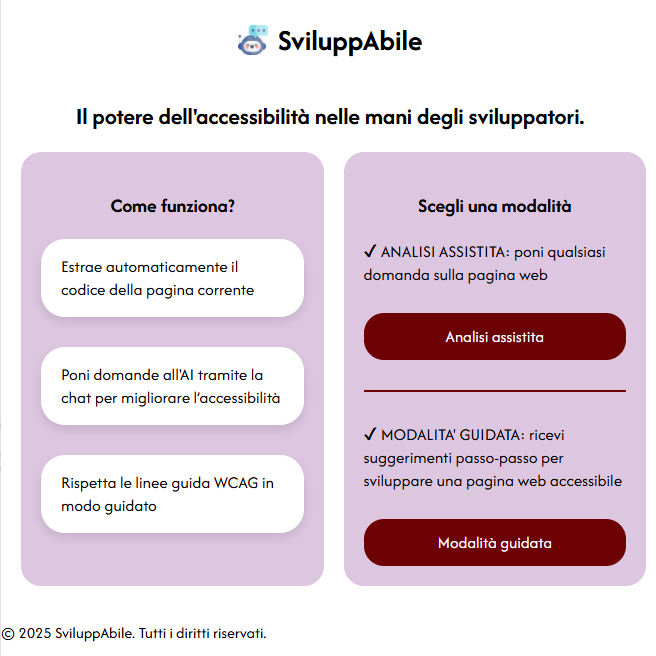
\includegraphics[width=0.6\linewidth, alt={Popup di avvio di \textit{SviluppAbile}}]{img/popup.png}}
    \caption{Popup di avvio dell'estensione \textit{SviluppAbile}}\label{fig:popup}
\end{figure}

\noindent Questa scelta iniziale permette all’utente di adattare lo strumento al proprio flusso di lavoro: analizzare passo-passo una pagina già esistente o sviluppare in maniera assistita un nuovo contenuto.

\subsubsection{Analisi assistita}
\noindent Nella modalità di analisi assistita (vedi figure \ref{fig:aass} e \ref{fig:aass_notte}), l’interfaccia dell’estensione si presenta suddivisa in due pannelli principali: sulla sinistra viene visualizzato il \acrshort{dom} della pagina web analizzata, mentre sulla destra compare la finestra della chat. Quest’ultima, inizialmente vuota, offre già due domande (\textit{"Come posso migliorare l'accessibilità della pagina web?"} e \textit{"Il mio codice rispetta le linee guida WCAG?"}), pensate per orientare l’utente nel primo utilizzo e stimolare un’interazione immediata. Oltre a tali suggerimenti, è disponibile un campo di testo in cui l’utente può inserire manualmente le proprie domande o richieste di chiarimento.\\

\begin{figure}[H]
    \centering
    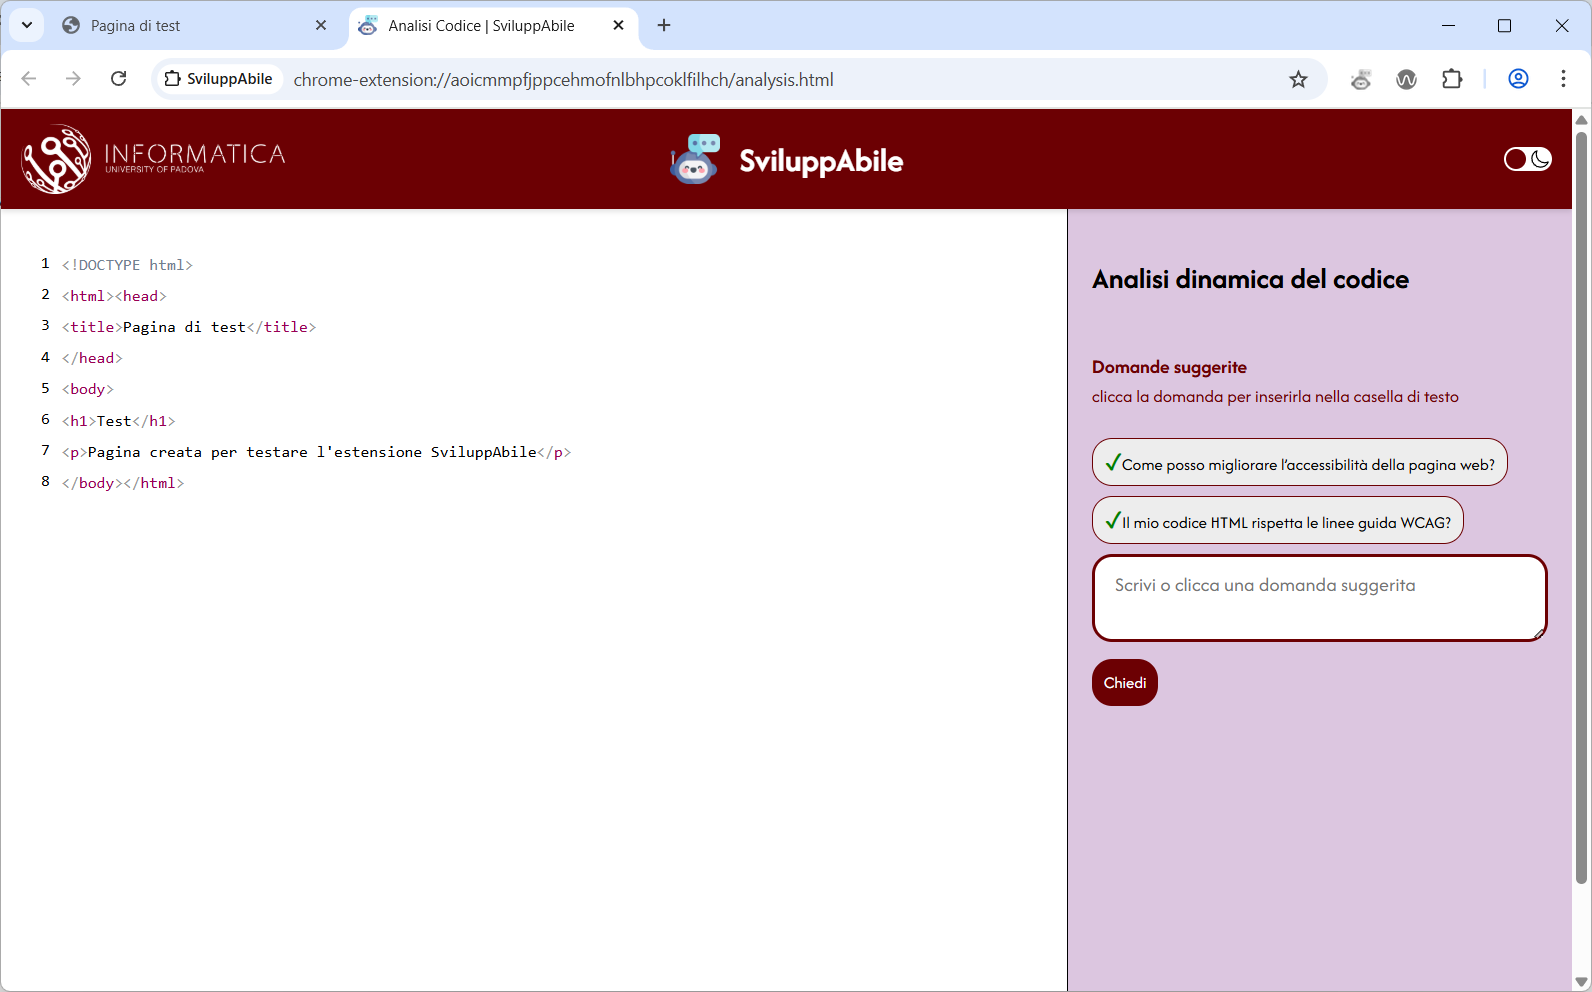
\includegraphics[width=1\linewidth, alt={Modalità di analisi assistita}]{img/analisi_ass.png}
    \caption{Modalità: analisi assistita}\label{fig:aass}
\end{figure}

\begin{figure}[H]
    \centering
    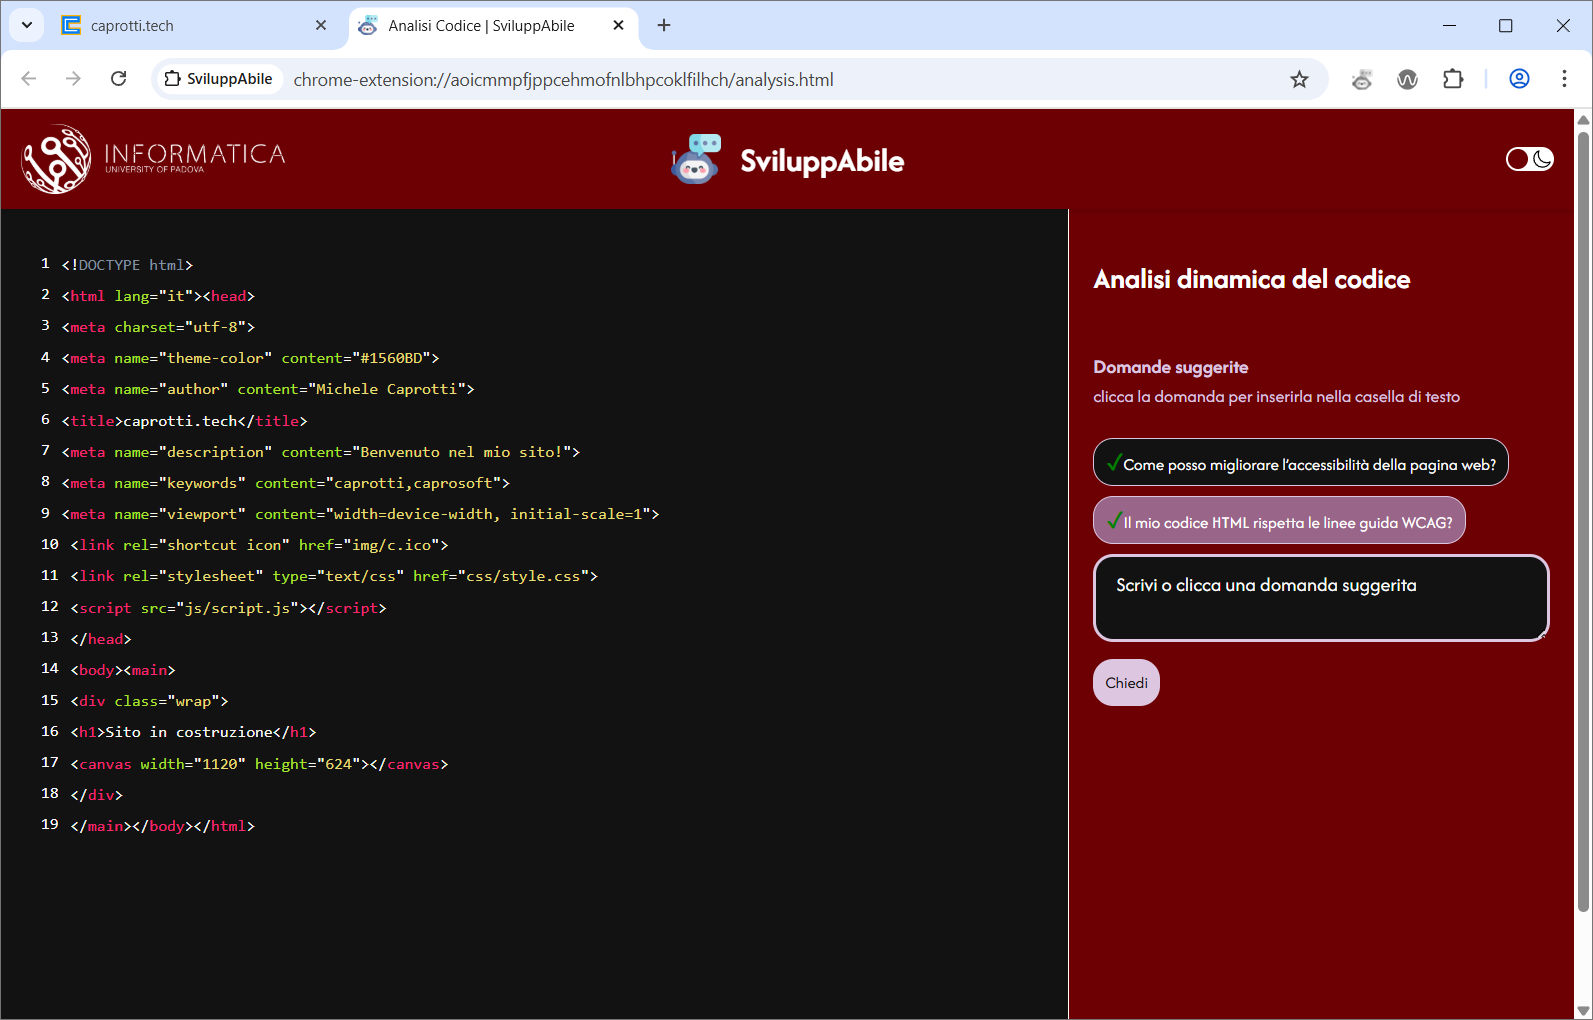
\includegraphics[width=1\linewidth, alt={Modalità di analisi assistita - modalità notturna}]{img/analisi_ass_dark.png}
    \caption{Modalità: analisi assistita - modalità notturna}\label{fig:aass_notte}
\end{figure}

\noindent L’interazione vera e propria inizia quando l’utente formula la prima domanda: a questo punto il \glslink{chatbotg}{chatbot} genera una risposta in linguaggio naturale, adattata al contesto del \acrshort{dom} analizzato. Per facilitare la comprensione delle spiegazioni, l’estensione è in grado di evidenziare automaticamente le porzioni di codice rilevanti all’interno del \acrshort{dom}, così da collegare visivamente l’errore o la soluzione proposta con la parte effettiva di codice interessata.\\
\\
Ad ogni scambio successivo, il sistema arricchisce la conversazione proponendo una o due nuove domande suggerite, collegate al tema trattato nella risposta precedente. Questa dinamica consente di mantenere la chat scorrevole e guidata, riducendo lo sforzo cognitivo dell’utente e favorendo un approccio progressivo alla comprensione delle problematiche di accessibilità della pagina web (vedi figura \ref{fig:aass2}).

\begin{figure}[H]
    \centering
    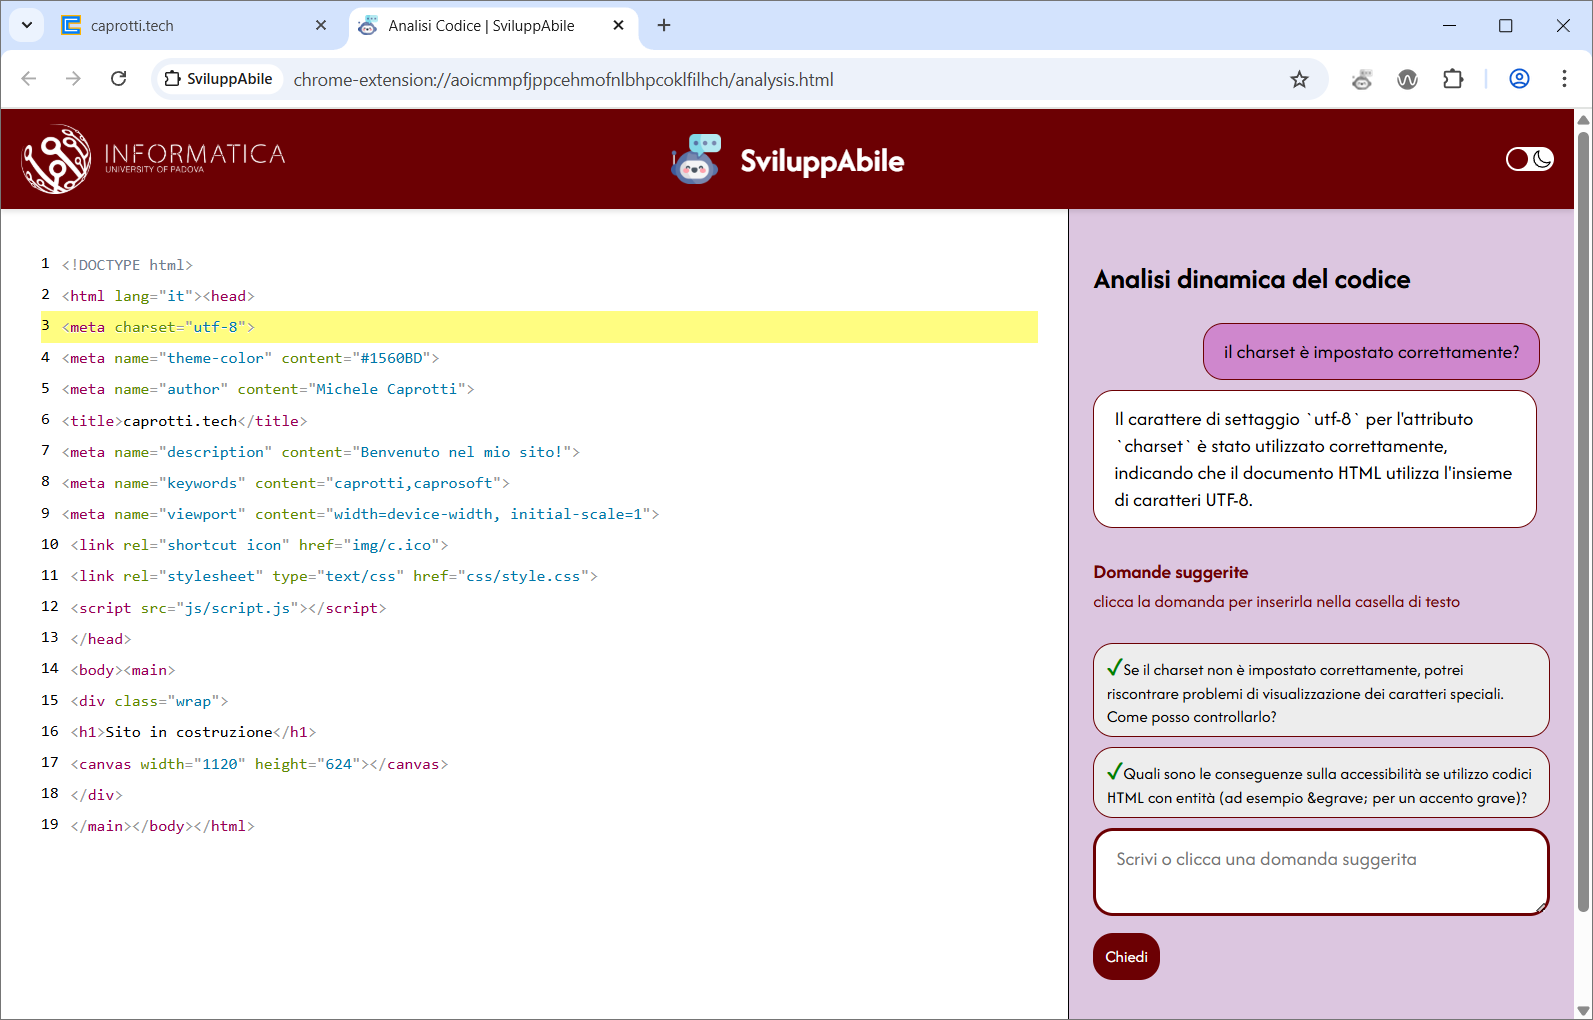
\includegraphics[width=1\linewidth, alt={Modalità di analisi assistita, dopo la prima interazione}]{img/analisi_ass2.png}
    \caption{Modalità: analisi assistita dopo un'interazione}\label{fig:aass2}
\end{figure}

\subsubsection{Modalità guidata}
\noindent La modalità di sviluppo guidato (vedi figure \ref{fig:mg} e \ref{fig:mg_notte}) si differenzia dall’analisi assistita per la presenza di un’interfaccia composta da tre pannelli distinti. Sulla sinistra rimane visibile il \acrshort{dom} della pagina mentre sulla destra è presente la finestra della chat. La novità è costituita dal pannello centrale, dedicato alla visualizzazione dei frammenti di codice suggeriti dal \glslink{chatbotg}{chatbot}.\\
\\
Inizialmente, quest’area centrale appare vuota e contiene soltanto un messaggio in grigio, con caratteri a richiamo “informatico”, che riporta la dicitura \texttt{eventuale codice suggerito}. Come nella modalità assistita, anche qui la chat propone due domande iniziali suggerite per avviare l’interazione: \textit{"Come si crea un <head> che contenga tutti gli elementi utili per una pagina accessibile?"} e \textit{"Come rendo accessibili le immagini?"}.\\

\begin{figure}[H]
    \centering
    \includegraphics[width=1\linewidth, alt={Modalità di sviluppo guidato}]{img/mg.png}
    \caption{Modalità: sviluppo guidato, pagina iniziale}\label{fig:mg}
\end{figure}

\begin{figure}[H]
    \centering
    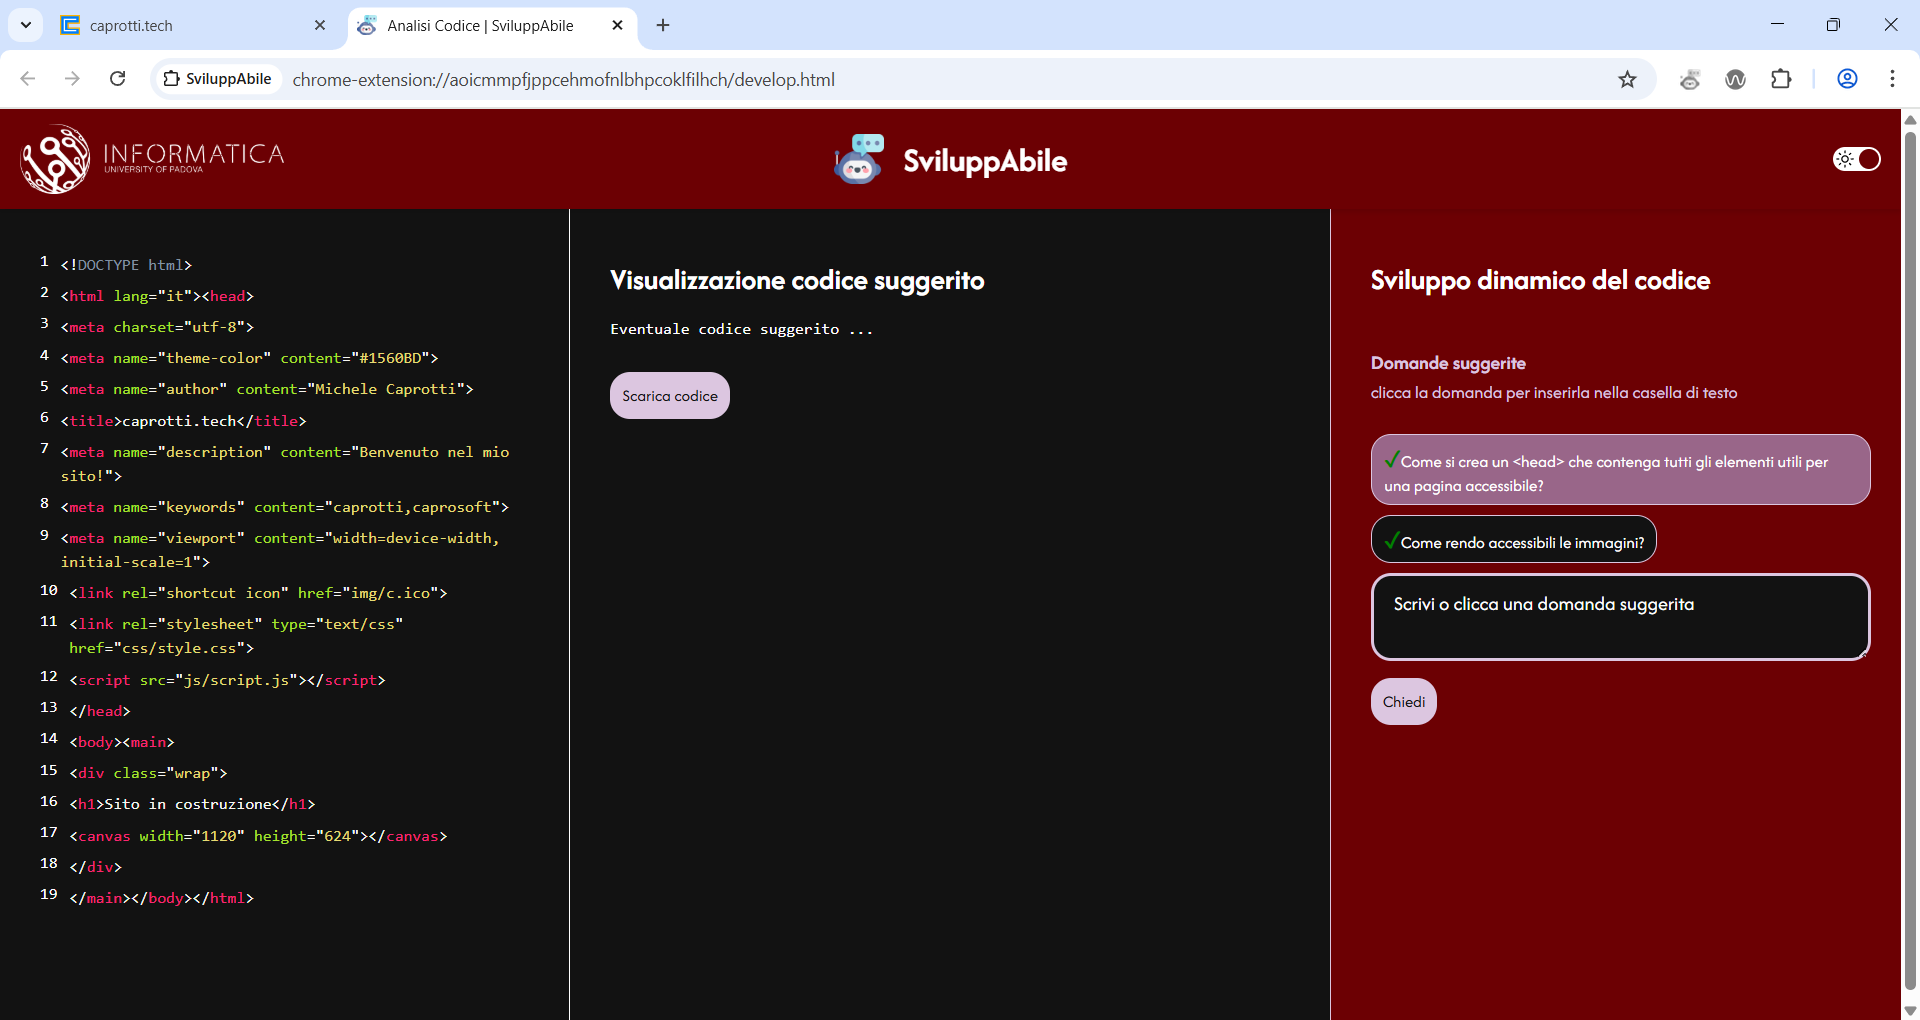
\includegraphics[width=1\linewidth, alt={Modalità di sviluppo guidato - modalità notturna}]{img/mg_dark.png}
    \caption{Modalità: sviluppo guidato - modalità notturna}\label{fig:mg_notte}
\end{figure}

\noindent Quando l’utente seleziona una domanda, il \glslink{chatbotg}{chatbot} non solo produce una risposta testuale, ma genera anche un blocco di codice che viene immediatamente visualizzato nel pannello centrale. Questa caratteristica rende la modalità guidata particolarmente utile in fase di sviluppo, poiché consente di osservare concretamente le soluzioni suggerite e di integrarle facilmente nel proprio progetto.\\
Per agevolare l’utilizzo pratico, ogni codice prodotto può essere scaricato direttamente tramite l’apposito pulsante “Scarica codice” (vedi figura \ref{fig:mg2}). L’estensione genera automaticamente un file \acrshort{html} contenente i blocchi di codice proposti, consentendo allo sviluppatore di salvare e riutilizzare le soluzioni in maniera rapida e strutturata.

\begin{figure}[H]
    \centering
    \includegraphics[width=1\linewidth, alt={Modalità di sviluppo guidato, dopo un'interazione}]{img/mg2.png}
    \caption{Modalità: sviluppo guidato, dopo alcune interazioni}\label{fig:mg2}
\end{figure}

\subsection{Interazione con l'AI}
\noindent L’estensione sviluppata prevede un’integrazione diretta con Ollama (come descritto in precedenza). Questa scelta garantisce all’utente il pieno controllo sui dati, riducendo i rischi legati alla trasmissione di informazioni sensibili verso servizi esterni e permettendo un utilizzo anche in assenza di connessione Internet stabile. L’interazione con l’\glslink{iag}{intelligenza artificiale} avviene attraverso chiamate HTTP ad un endpoint locale, al quale vengono inviati prompt costruiti dinamicamente in base alle esigenze del flusso operativo. Il codice \ref{lst:funzOllama} mostra tale interazione.

\begin{lstlisting}[style=jsStyle, caption={Funzione di interazione con Ollama}, label={lst:funzOllama}]
async function inviaPrompt(prompt) {
  const res = await fetch('http://localhost:11434/api/generate', {
    method: 'POST',
    headers: { 'Content-Type': 'application/json' },
    body: JSON.stringify({
      model: "llama3.1:8b",
      prompt,
      stream: false
    })
  });
  return await res.json();
}
\end{lstlisting}

\noindent Sono stati definiti tre casi d’uso principali per la generazione dei prompt: 
\begin{itemize}
    \item l’invio congiunto del \acrshort{dom} della pagina e della domanda dell’utente, utile per ricevere spiegazioni e indicazioni sulle righe che verranno poi evidenziate in quanto utili alla comprensione della risposta. Tale prompt è visibile nel codice \ref{lst:rr}; 
    \begin{lstlisting}[style=jsStyle, caption={Prompt per la generazione di risposta e righe da evidenziare}, label={lst:rr}]
    const promptPrincipale =
    `Sei un assistente che analizza codice HTML. Rispondi alla domanda in modo chiaro ma conciso, usando al massimo 5-6 frasi. ` +
    `Evita ripetizioni o spiegazioni troppo generiche. ` +
    `Alla fine della risposta, su una nuova riga, scrivi le righe eventualmente utilizzate per la risposta nel seguente formato:\n\n` +
    `##RIGHE##\n{"righe": [elenco_di_numeri_di_riga]}\n\n` +
    `Codice HTML:\n${codice}\n\nDomanda: ${domanda}`;
    \end{lstlisting}
    
    \item l'invio della sola domanda per generare ulteriori domande più approfondite da consigliare all'utente, come visibile nel codice \ref{lst:dsucc};
    \begin{lstlisting}[style=jsStyle, caption={Prompt per la generazione di domande successive}, label={lst:dsucc}]
    const promptSuccessiva =
    `Suggerisci 1 o 2 domande piu' specifiche sull'accessibilita' o sull'analisi del codice, ` +
    `partendo dalla seguente domanda:\n\n` +
    `Rispondi solo con il seguente formato JSON:\n\n` +
    `##DOMANDA##\n{ "domande": ["prima domanda", "seconda...", "terza..."] }\n\n` +
    `Domanda iniziale: ${domanda}`;
    \end{lstlisting}

    
    \item l’invio del \acrshort{dom} insieme alla richiesta di modifica, scenario in cui l’\acrshort{ia} produce sia una risposta argomentata sia un blocco di codice pronto per essere inserito nel pannello centrale della pagina nella modalità di sviluppo guidato (vedi codice \ref{lst:rc}).
    \begin{lstlisting}[style=jsStyle, caption={Prompt per la generazione di risposta e codice \acrshort{html} accessibile}, label={lst:rc}]
    const promptCodice =
      `Sei un assistente che aiuta a rendere accessibile il codice HTML. ` +
      `Rispondi in massimo 5-6 frasi chiare e tecniche. ` +
      `Se suggerisci del codice, racchiudilo tra i marcatori \`##CODICE##\` come mostrato di seguito:\n\n` +
      `##CODICE##\n<codice HTML da inserire o modificare>\n##FINECODICE##\n\n` +
      `Codice HTML:\n${codice}\n\nDomanda: ${domanda}`;
    \end{lstlisting}

\end{itemize}
Questa diversificazione consente di mantenere un approccio modulare e adattabile, rendendo l’assistente in grado di rispondere a necessità differenti con un unico modello sottostante.


\subsection{Filtraggio risposta generata}
\noindent Un aspetto fondamentale del funzionamento dell'estensione riguarda il filtraggio e la rielaborazione della risposta generata dall’intelligenza artificiale. Le risposte restituite da Ollama, infatti, non vengono mostrate direttamente all’utente, ma sono sottoposte ad un processo di \glslink{parsingg}{parsing\glox} e di pulizia.\\
In primo luogo, l’estensione distingue le diverse tipologie di output attese: la risposta vera e propria alla domanda inserita, le eventuali domande suggerite e gli eventuali blocchi di codice generati da visualizzare e/o scaricare. A tal fine vengono utilizzati marcatori testuali inseriti nel prompt (ad esempio \texttt{\#\#DOMANDE\#\#} o \texttt{\#\#CODICE\#\#}), che consentono di individuare con precisione le sezioni rilevanti all’interno della risposta. \\Una volta ricevuto l’output, funzioni dedicate come \texttt{estraiRigheDaRisposta} ed \\ \texttt{estraiDomandeSuggerite} applicano espressioni regolari per isolare le parti utili, scartando elementi ridondanti o formattazioni non necessarie.\\
\\
Il filtraggio consente anche di separare le informazioni in blocchi distinti, in modo che ciascun contenuto possa essere mostrato nella pagina web nel pannello appropriato (ad esempio, suggerimenti testuali nella chat e codice sorgente nel riquadro centrale). Questo approccio riduce il carico cognitivo per l’utente, che non si trova di fronte a una risposta grezza e complessa, ma ad un output strutturato e facilmente navigabile.\\ Inoltre la possibilità di visualizzare alcune righe di codice evidenziate consente una comprensione più immediata del codice sorgente analizzato rendendo più intuitivo il processo di revisione del codice.

\section{Problematiche riscontrate}
\noindent Durante lo sviluppo del progetto sono emerse alcune criticità di natura tecnica. In primo luogo, la scelta dell’\acrshort{ia} da integrare si è rivelata complessa: le \acrshort{api} gratuite disponibili online presentavano forti limitazioni legate al numero di token, rendendole inadeguate per un utilizzo continuativo. Successivamente è stata valutata l’adozione di Ollama, la cui installazione, tuttavia, non è risultata possibile sul computer personale a causa delle risorse hardware insufficienti. L’ostacolo è stato superato grazie alla disponibilità di un computer fornito dall’università, che ha consentito l’utilizzo stabile della piattaforma.\\\\
Un’ulteriore problematica si è manifestata dopo l’integrazione dell’\acrshort{ia} nell’estensione: l’invio delle richieste tramite la chat restituiva sistematicamente il messaggio \texttt{“Errore durante l’elaborazione: Risposta vuota dal server”}. Attraverso un’attenta fase di \glslink{debuggingg}{debug}, supportata dall’inserimento di log per tracciare l’esecuzione, è stato possibile individuare la causa: non un malfunzionamento dell’\acrshort{ia} o dell'estensione, bensì le restrizioni imposte da Chrome, che limitano l’interazione delle estensioni con \acrshort{api} esterne, bloccando di fatto la corretta trasmissione delle richieste. Tale problema è stato risolto avviando Chrome da terminale con parametri specifici che disabilitano i blocchi di sicurezza predefiniti, permettendo così all’estensione di comunicare correttamente con l’\acrshort{ia}.\\
\noindent Ecco il comando utilizzato: 
\begin{verbatim} 
  chrome.exe --disable-web-security --user-data-dir="C:_temp_chrome" 
\end{verbatim}

\noindent Per evitare l’uso di tale comando, è necessario impostare correttamente alcune variabili di sistema su Windows per l’utilizzo di LLaMA 3.1:8B come estensione di Chrome: 
\begin{verbatim} 
  OLLAMA_HOST = 0.0.0.0 
  OLLAMA_ORIGINS = chrome-extension://* 
\end{verbatim} 

\vspace{0.3cm}
\noindent Infine, è emersa una limitazione legata alla gestione della memoria dell’\acrshort{ia}: idealmente, il codice sorgente della pagina avrebbe potuto essere caricato una sola volta al momento della scelta della modalità, inviando in seguito soltanto le domande per migliorare tale codice. \\Tuttavia, Ollama non dispone di una capacità di memoria sufficiente a mantenere lo stato della conversazione in assenza del ricaricamento completo del \acrshort{dom}. Ciò comporta la necessità di reinviare l’intero contenuto ad ogni interazione, con un impatto significativo sull’efficienza complessiva.
